%% LaTeX2e class for student theses
%% thesis.tex
%% 
%% Karlsruhe Institute of Technology
%% Institute for Program Structures and Data Organization
%% Chair for Software Design and Quality (SDQ)
%%
%% Dr.-Ing. Erik Burger
%% burger@kit.edu
%%
%% Version 1.1, 2014-11-21

%% Available languages: english,ngerman
%% Available modes: draft,final (see README)
\documentclass[ngerman,draft]{sdqthesis}

%% ---------------------------------
%% | Information about the thesis  |
%% ---------------------------------

%% Name of the author
\author{Thomas Czogalik}

%% Title (and possibly subtitle) of the thesis
\title{Datenflussmodellierung für\\
Vertraulichkeitsanalysen in Palladio}

%% Type of the thesis 
\thesistype{Proposal für die Bachelorarbeit}

%% Change the institute here, ``IPD'' is default
% \myinstitute{Institute for \dots}

%% You can put a logo in the ``logos'' directory and include it here
%% instead of the SDQ logo
% \grouplogo{myfile}
%% Alternatively, you can disable the group logo
% \nogrouplogo

%% The reviewers are the professors that grade your thesis
\reviewerone{Prof. Dr. Ralf H. Reussner}
\reviewertwo{Jun.-Prof. Dr.-Ing. Anne Koziolek}

%% The advisors are PhDs or Postdocs
\advisorone{M. Sc. Stephan Seifermann}
%% The second advisor can be omitted
\advisortwo{Dipl.-Inform. Emre Taşpolatoğlu}

%% Please enter the start end end time of your thesis
\editingtime{01. Juni 2016}{31. September 2016}

\settitle

%% --------------------------------
%% | Settings for word separation |
%% --------------------------------

%% Describe separation hints here.
%% For more details, see 
%% http://en.wikibooks.org/wiki/LaTeX/Text_Formatting#Hyphenation
\hyphenation{
% me-ta-mo-del
}

%% --------------------------------
%% | Bibliography                 |
%% --------------------------------

%% Use biber instead of BibTeX, see README
\usepackage[citestyle=numeric,style=numeric,backend=biber]{biblatex}
\addbibresource{thesis.bib}

%% ====================================
%% ====================================
%% ||                                ||
%% || Beginning of the main document ||
%% ||                                ||
%% ====================================
%% ====================================
\begin{document}

%% Set PDF metadata
\setpdf

%% Set the title
\maketitle

%% The Preamble begins here
\frontmatter

%%% LaTeX2e class for student theses: Declaration of independent work
%% sections/declaration.tex
%% 
%% Karlsruhe Institute of Technology
%% Institute for Program Structures and Data Organization
%% Chair for Software Design and Quality (SDQ)
%%
%% Dr.-Ing. Erik Burger
%% burger@kit.edu
%%
%% Version 1.1, 2014-11-21

\thispagestyle{empty}
\null\vfill
\noindent\hbox to \textwidth{\hrulefill} 
\iflanguage{english}{I declare that I have developed and written the enclosed
thesis completely by myself, and have not used sources or means without
declaration in the text.}%
{Ich versichere wahrheitsgemäß, die Arbeit
selbstständig angefertigt, alle benutzten Hilfsmittel vollständig und genau
angegeben und alles kenntlich gemacht zu haben, was aus Arbeiten anderer
unverändert oder mit Änderungen entnommen wurde.}
 
 
%% ---------------------------------------------
%% | Replace PLACE and DATE with actual values |
%% ---------------------------------------------
\textbf{PLACE, DATE}
\todo{Please replace with actual values}
\vspace{1.5cm}
 
\dotfill\hspace*{8.0cm}\\
\hspace*{2cm}(\theauthor) 
\cleardoublepage

\setcounter{page}{1}
\pagenumbering{roman}


%% ------------------------
%% |   Table of Contents  |
%% ------------------------
\tableofcontents

%\listoffigures
%\listoftables

%% -----------------
%% |   Main part   |
%% -----------------

\mainmatter

%% LaTeX2e class for student theses
%% sections/content.tex
%% 
%% Karlsruhe Institute of Technology
%% Institute for Program Structures and Data Organization
%% Chair for Software Design and Quality (SDQ)
%%
%% Dr.-Ing. Erik Burger
%% burger@kit.edu
%%
%% Version 1.1, 2014-11-21

\chapter{Einleitung}
\label{ch:Einleitung}
Heutige IT-Systeme verarbeiten immer mehr vertrauliche Daten und werden gleichzeitig komplexer. Die Vertraulichkeit der Daten soll innerhalb der Komponenten, auf dem jeweiligen Gerät sowie beim Übertragen zwischen Software"=Komponenten oder Geräten gewährleistet werden. Dies ist eine große Herausforderung. Außerdem ist eine Bewertung, ob das System ausreichend abgesichert ist schwierig, da in komplexen Systemen unklar ist, wo relevante Daten verarbeitet werden. \par
Dies ist mithilfe von Datenflussanalysen möglich. Diese Analysen nutzen die Implementierung der Anwendung als Eingabe. Fehler können dadurch aber erst nach der Implementierung erkannt und nicht bereits vorzeitig beseitigt werden. Ist ein Fehler durch eine mangelhafte Architektur entstanden, muss ggf. sogar ein Großteil der Implementierung verworfen werden. Ansätze zum Erkennen solcher Fehler auf Architekturebene sind in Entwicklung, aber scheitern daran, dass Datenflüsse auf Architekturebene bisher nur indirekt, zum Beispiel über Parameterübergabe spezifizierbar sind. \\
%Motivation: \\
%Vertrauliche Daten die in verteilten SoftwareSystemen bergen sicherheitsrisiko \\
%- ausgetauscht zwischen logischen komponenten, physikalischen geräten, Protocol Stack / Stapel \\
%Datenlecks auf implementierungsebene fixen ist teuer \\
%- nicht nur source code sondern evtl architektur muss überdenkt werden.\\
%Datenfluss von vertraulichen daten bereits beim system design beachten \\
%Dabei können verletzungen des Datenschutzrechts oder der anforderungen an externe dienstleister auf architektur ebende erkannt werden \\

Ziel dieser Bachelorarbeit ist die Modellierung von Datenflüssen auf Architekturebene zu ermöglichen. Diese Modellierung soll für eine Vertraulichkeitsanalyse in Palladio genutzt werden. Sie soll aber auch für andere auf Datenflüssen aufbauende Analysen, beispielsweise aus dem Sicherheitsbereich nutzbar sein. \par
Nachdem der Datenfluss modelliert wurde, soll es möglich sein sicherheitsrelevante Eigenschaften zu definieren.
%Zum Beispiel die Eigenschaft das bestimmte Daten nicht mit anderen Daten zusammenkommen dürfen, da sonst die Vertraulichkeit gefährdet wäre. \\
Auch der Standort der Hardware soll spezifizierbar sein. Dabei soll verhindert werden, dass die Vertraulichkeit der Daten gefährdet wird, wenn diese an einen Ort geraten, an dem Vertraulichkeit nicht garantiert werden kann. \\
Außerdem soll die Möglichkeit gegeben werden Verbindungen zwischen Komponenten oder Geräten zu charakterisieren, beispielsweise dadurch, ob auf der Verbindung die Daten verschlüsselt übertrage werden oder nicht. \\
%Sollte nicht sicher sein, ob es sich um eine Verletzung der Vertraulichkeit handelt, soll die Analyse dem Benutzer Feedback gebe, damit dieser entscheidet was zu tun ist. \\
%Ziele: \\
%Allgemeine Vertraulichkeitsanalyse auf Architekturebene modelieren \\
%Im anschluß für palladio implementieren \\
%%Ziel der Analyse: Datenlecks vermeiden \\
%Erkenne ob Daten sich gegenseitig beeinflussen \\
%Analyse beachtet Standort (HW) \\
%Analyse gibt kritische Stellen an Benutzer weiter \\

%%Erweiterbarkeit (SEFF Aktionen (zu Beginn z.B. lesen, kombinieren, schreiben))
%%Vorgehen:\\
%%Vertraulichkeit spezifizieren und analysieren \\
%%abstrakte syntax -> Meta modell -> daten und DF modelieren \\
%%- DF wird innerhalb von Komponenten modelliert (SEFF) \\
%%Daten sollen über Schnittstellen ausgetauscht werden (Palladio Signaturen) \\
Im folgenden Kapitel \ref{ch:Grundlagen} werden die Grundlagen erläutert, die für die geplante Bachelorarbeit benötigt werden. In Kapitel \ref{ch:VerwandteArbeiten} wird ein Überblick über verwandte Arbeiten gegeben. Die geplanten Tätigkeiten der Bachelorarbeit werden in Kapitel \ref{ch:Konzeption} beschrieben. Die Beschreibung der Validierung erfolgt in Kapitel \ref{ch:Validierung}. In den Kapiteln \ref{ch:Organisatorisches} und \ref{ch:Zeitplan} werden die Organisation und der Zeitplan sowie Risikomanagement erläutert.
%Struktur: \\
%Grundlagen in Sec 2 \\
%Verwandte Arbeiten Sec 3\\
%KOnzeption der BA Sec 4 \\
%Validierung der BA mithilfe einer Analyse Sec 5 \\
%Organisatorische Sec 6 \\
%Risikomanegemnet Sec 7\\
%% LaTeX2e class for student theses
%% sections/conclusion.tex
%% 
%% Karlsruhe Institute of Technology
%% Institute for Program Structures and Data Organization
%% Chair for Software Design and Quality (SDQ)
%%
%% Dr.-Ing. Erik Burger
%% burger@kit.edu
%%
%% Version 1.1, 2014-11-21

\chapter{Grundlagen}
\label{ch:Grundlagen}
Im folgenden Abschnitt werden grundlegende Konzepte und Begriffe erläutert, die für die geplante Bachelorarbeit benötigt werden.
\section{Vertraulichkeit}
In der Literatur gibt es verschiedene Definitionen für Vertraulichkeit. In der Europäischen-Datenschutzgrundverordnung (EU-DSGVO) heißt es, dass Vertraulichkeit die Eigenschaft ist, dass Unbefugte keinen Zugang zu den Daten haben und weder die Daten noch die Geräte, mit denen diese verarbeitet werden, benutzen können (vgl. Art. 26ff EU-DSGVO). 
Eine andere Definition liefert das Bundesverfassungsgericht (BVerfG) in einem Urteil. Laut diesem versteht man unter Vertraulichkeit den Schutz vorhandener Daten gegen das Ausspähen (vgl. BVerfG 120, 274). Eine weitere Definition findet sich in dem Buch \textbf{Secure Systems Development with UML} \cite{Jurjens2005}. Dort heißt es, dass Daten nur von legitimen Parteien gelesen werden dürfen.
Eine Festlegung auf einen Vertraulichkeitsbegriff soll hier noch nicht geschehen. Dies soll im Zuge der Spezifizierung der Vertraulichkeit (vgl. \ref{subch:SpezifiziereVertraulichkeit}) als eigenständige Arbeit geschehen.

%%Definitionen: (sortieren: europäischer als oberdefinition, Bverfg und umlsec als spezifikation \\
%%-Daten dürfen nur von legitimen Parteien gelesen werden \\
%%-Schutz vor unbefugter Preisgabe von Informationen an dritte (IT Wissen)\\
%%-unbefugte kein zugang zu Daten und geräten(europäischer Datenschutz) \\
%%- Schutz vorhandener Daten gegen Ausspähen (BVerfG 2008, [11 Abs 180])


\section{Modellgetriebene Software-Entwicklung}
In der modellgetriebenen Software-Entwicklung \cite{Stahl2007} werden Teile des Software-Systems mit Hilfe von Modellen auf einem höheren Abstraktionslevel beschrieben. Dabei fließen die Modelle in die Software mit ein und sind Teil des Endproduktes. Das Ziel der modellgetriebenen Softwareentwicklung ist die Verbesserung der Softwarequalität und der Wiederverwendbarkeit. Außerdem soll eine Erhöhung der Entwicklungseffizienz zum Beispiel durch Quellcodeerzeugung aus den Modellen erreicht werden. 
\subsection{Modell}
\label{subch:Modell}
Nach Herbert Stachowiak \cite{Stachowiak1973} zeichnet sich ein Modell durch die folgenden drei Merkmale aus.
\begin{itemize}
\item \textbf{Abbildung} - Bei einem Modell handelt es sich um eine Abbildung oder Repräsentation von einem künstlichen oder natürlichen Original. Das Original kann selbst wieder ein Modell sein. 
\item \textbf{Verkürzung} - Es werden nicht alle Attribute des Originals erfasst, sondern nur diejenigen, die relevant sind.
\item \textbf{Pragmatismus} - Modelle erfüllen ihre Ersatzfunktion für bestimmte Subjekte, innerhalb einer bestimmten Zeit und unter Einschränkung bestimmter gedanklicher oder tätlicher Operationen. Beispielsweise benötigt eine Analyse je nach gewünschter Genauigkeit auch unterschiedlich genaue Modelle. Der Pragmatismus schreibt vor, dass man hier nicht unnötig genau arbeitet.
\end{itemize} 
Ein Original könnte zum Beispiel eine Audio-Datei sein und das dazugehörige Modell könnte ein Lied-Element mit Titel "'Stairway to Haven"', des Sängers "'Led Zeppelin"' und dem Jahr "'1971"' sein.

\subsection{Meta-Modelle}
Ein Meta-Modell beschreibt die Struktur eines Modells. In dem Musik-Beispiel, würde das Meta-Modell eine Klasse \textbf{Song} mit den Attributen \textbf{Titel}, \textbf{Sänger}, vom Typ String und \textbf{Jahr} vom Typ Integer enthalten.
Ein Meta-Modell muss folgende Bereiche abdecken:
\begin{itemize}
\item \textbf{Abstrakte Syntax}: Sie beschreibt die Konstrukte, aus denen die Modelle bestehen, sowie deren Eigenschaften und Beziehungen.
\item \textbf{Konkrete Syntax}: Diese beschreibt die Darstellung der Konstrukte, Eigenschaften und Beziehungen, die in der abstrakten Syntax spezifiziert sind.
\item \textbf{Statische Semantik}: Mithilfe dieser werden Modellierungsregeln und Einschränkungen ausgedrückt, die mit der abstrakten Syntax nicht möglich sind.
\item \textbf{Dynamische Semantik}: Sie drückt die Bedeutung der Konstrukte aus und wird oft nicht formal, sondern durch natürlichsprachlichen Text spezifiziert.
\end{itemize}

\section{Rollen der komponentenbasierten Entwicklung} \label{sec:rolls}
Die Modellierung des Datenflusses erfolgt auf Software-Architektur-Modellen. Dabei gibt es vier verschiedene Rollen \cite{Koziolek2006}, die an unterschiedlichen Teilen der Architektur arbeiten und dort ihr spezifisches Wissen einbringen.
\begin{itemize}

\item \textbf{Systemarchitekt}: Die Architektur und der Zusammenhang der einzelnen Komponenten miteinander werden vom Systemarchitekten entworfen. Er ist auch dafür zuständig weitere Anweisungen an die anderen Rollen weiterzugeben.
\item \textbf{Domänenxperte}: Das Wissen darüber, wie der Benutzer mit dem System interagiert und welche Parameter im Kontrollfluss verwendet werden, stammt vom Domänenxperten.
\item \textbf{Komponentenentwickler}: Für das Implementieren und Spezifizieren der einzelnen Komponenten ist der Komponentenentwickler verantwortlich.
\item \textbf{Softwareverteilungsexperte}: Die Zusammenstellung der Systemumgebung der Software wird vom Softwareverteilungsexperten übernommen. Außerdem weist der Softwareverteilungsexperte den Komponenten Ressourcen zu.

\end{itemize}

\section{Palladio Komponentenmodell (PCM)}
Das Palladio Komponentenmodell (PCM) \cite{Becker2010} ist eine Architecture-Description-Language (ADL). Sie wird verwendet um komponentenbasierte Software zu beschreiben. Neben der Beschreibung sind auch Qualitätsanalysen, wie etwa bezüglich der Performanz oder Zuverlässigkeit möglich. Im Folgenden werden Teile des PCM erklärt, die für die Bachelor Arbeit wichtig sind.

\subsection{Submodelle}
Auch im PCM werden vier Rollen betrachtet. Diese entsprechen den Rollen aus \ref{sec:rolls}. Der einzige Unterschied ist dabei, dass im PCM der Systemarchitekt Software-Architekt heißt. Die Aufgaben sind jedoch die selben.  \\
Jede dieser Rollen ist außerdem für ein bestimmtes Submodell zuständig.
Für das \textbf{Component"=Repository-Modell} ist der Komponentenentwickler zuständig. Dieses Modell enthält die einzelnen Komponenten und Schnittstellen. Der Software-Architekt ist für das \textbf{System-Modell} zuständig, das die Zusammensetzung der Komponenten charakterisiert. Der Softwareverteilungsexperte ist für gleich zwei Modelle verantwortlich. Das erste Modell, ist das \textbf{Execution-Environmet-Modell}. Es beschreibt die benutzte Hardware und das Netzwerk. Das zweite Modell beschreibt wie die einzelnen Komponenten auf der Hardware verteilt werden. Dieses Modell ist das \textbf{Component-Allocation-Modell}. Schließlich ist der Domänenxperte für das \textbf{Usage-Modell} zuständig. Dieses beschreibt die Interaktion des Benutzers mit dem System. \\
Diese Modelle werden im Rahmen der Bachelorarbeit entsprechend um die Möglichkeit zur Modellierung von Datenflüsse und ggf. weiteren für die Vertraulichkeitsanalyse notwendigen Eigenschaften erweitert.

\subsection{Service Effect Specification (SEFF)}
Mithilfe der Service Effect Specification (SEFF) \cite{Reussner} kann das Verhalten innerhalb der Komponenten auf abstrakten, auf bestimmte Qualitätsattribute zugeschnittenen Leveln beschrieben werden. 
Durch das spezifizieren von SEFFs kann man die Software auf Architekturebene analysieren. Dabei gibt es drei verschiedene Abstraktionslevel, die aufeinander aufbauen:
\begin{itemize}
\item \textbf{Signature-List-Based-Interface}: Schnittstellen dienen zur Kommunikation zwischen den Komponenten. Auf dem Signature-List-Based-Interface bauen die anderen Abstraktionslevel auf. Es besteht aus Parametern und Rückgabewerten.
\item \textbf{Protocol-Modeling-Interface}: Mithilfe dieser Schnittstelle lassen sich Aufrufsequenzen definieren.
\item \textbf{Quality-Of-Service-Modelling Interface}: Hier können verschiedene Qualitätsattribute definiert werden.
\end{itemize}
Der RDSEFF ist eine Erweiterung der SEFF. Die Performanzvorhersage für Komponenten basiert in Palladio unter anderem auf der Notation des RDSEFFs. \\
Im Rahmen der Bachelorarbeit soll eine weitere SEFF-Spezialisierung entstehen, die den Datenfluss innerhalb der Komponenten beschreibt.

%performance unabhängig \\
%abstrakte syntax \\
%beschreibt Verhalten innerhalb der Komponenten \\
%abstraktes Level \\
%erlaubt analyse auf Architektur ebene \\
%abstraktions level hängt von Analyse ab \\
%3 Level \\
%%- Signature list based Interface \\
%- protocol-modeling interface \\
%- Quality of Service modeling interface \\

%Ressource Demanding Seff als beispiel einer implementierung -> data flof seff



%% LaTeX2e class for student theses
%% sections/conclusion.tex
%% 
%% Karlsruhe Institute of Technology
%% Institute for Program Structures and Data Organization
%% Chair for Software Design and Quality (SDQ)
%%
%% Dr.-Ing. Erik Burger
%% burger@kit.edu
%%
%% Version 1.1, 2014-11-21

\chapter{Verwandte Arbeiten}
\label{ch:VerwandteArbeiten}
Im Folgenden werden Arbeiten vorgestellt, die ähnliche Aufgabenstellungen haben oder Teile der Bachelorarbeit behandeln. \\

Für die Spezifizierung der Vertraulichkeit in Abschnitt \ref{subch:SpezifiziereVertraulichkeit} werden die folgenden Arbeiten verglichen um die verschiedenen Aspekte von Vertraulichkeit zu beleuchten und notwendige Eingabedaten für Vertraulichkeitsanalysen zu ermitteln.
\begin{itemize}
\item In der erste Arbeit \textbf{Specification and Verification of
Confidentiality in Component"=Based Systems} \cite{Kramer} wird Vertraulichkeit spezifiziert indem Anforderungen aufgestellt werden, die von einem vertraulichen System erfüllt werden müssen.
\item In dem Buch \textbf{Secure System Development for UML} \cite{Jurjens2005} werden zunächst einige Sicherheitseigenschaften spezifiziert (unter anderem Vertraulichkeit) um eine Sicherheitsanalyse für UML-Diagramme durchführen zu können.
\item In der Arbeit \textbf{A Security Confidential Document Model and Its Application} \cite{Zheng2010} wird ein Model vorgestellt, mit dem die Vertraulichkeit von elektronischen Dokumenten sichergestellt werden soll. Hier werden auch Anforderungen für Vertraulichkeit spezifiziert.
\end{itemize}

In dem Buch \textbf{Principles of Program Analysis} \cite{Nielson1999} wird die Datenflussanalye auf Implementierungsebene beschrieben. Obwohl in der Bachelorarbeit Datenflüsse auf Architekturebene betrachtet werden, kann das Buch als Grundlagenlektüre für Datenflussanalysen dienen. \\
In der Arbeit \textbf{Model-Driven Specification and Analysis of Confidentiality in Component"=Based Systems} \cite{Kramera} werden Datenflüsse auf Architekturebene betrachtet, aber nicht innerhalb der Komponenten. Im Laufe der Bachelorarbeit soll die dort erarbeite Vertraulichkeitsanalyse für die Validierung (vgl. Kapitel \ref{ch:Validierung}) dienen. \\

Außerdem konnten drei Paladio-Erweiterungen identifiziert werden, die sich mit dem Problem der Datenflussmodellierung befassen.
\begin{itemize}
\item \textbf{Model-Driven Specification and Analysis of Confidentiality in Component"=Based Systems} \footnote{\url{https://sdqweb.ipd.kit.edu/wiki/Model-Driven_Specification_and_Analysis_of_Confidentiality_in_Component-Based_Systems}} ist eine Erweiterung, die die Vertraulichkeit von Informationen spezifiziert und analysiert, die in komponentenbasierten Systemen verarbeitet werden
\item \textbf{PASE} \footnote{https://sdqweb.ipd.kit.edu/wiki/PASE} erlaubt in PCM-Modellen den Datenfluss zu modellieren und analysieren.
\item \textbf{Palladio.TX} \footnote{https://sdqweb.ipd.kit.edu/wiki/Palladio.TX} modelliert und analysiert transaktionale Informationssysteme und spezifiziert dazu Daten, sowie deren Speicherung in Datenbanktabellen.
\end{itemize}
Die drei Erweiterungen liefern jedoch keine oder keine ausreichende Dokumentation. Nur \textbf{PASE} liefert auf seiner Wiki-Seite eine Beschreibung der Erweiterung des Metamodells. Außerdem kann keine der Erweiterungen feststellen, wie Daten innerhalb von Komponenten verarbeitet werden. Dies ist jedoch für eine Vertraulichkeitsanalyse notwendig.
 
%erwähne Palladion Erweiterungen und Grenze dich ab (können z.B. nicht feststellen, welche %Parameter sich beeinflussen) \\

%Für Modellierung und Spezifizierung: Poster: Specification and Veri?cation of Confidentiality in Component-Based Systems \\
%Secure System Development with UML

%Für Analyse: Architectural Data Flow Analysis, Stephan; Poster: Specification and Verification of Confidentiality in Component-Based Systems \\
%Datenflussanalyse implementierung vs architektur \\
%untersuche zwischen welchen Teilen Daten weitergegeben werden --> welche Abhängigkeiten entstehen \\
%mithilfe controll flow graph (CFG) \\
%CFG besteht aus Codeblöcken \\
%Einzelne Blöcke werden untersucht, wie Daten sich im Block verändern, bzw. zwischen Blöcken \\
%% LaTeX2e class for student theses
%% sections/content.tex
%% 
%% Karlsruhe Institute of Technology
%% Institute for Program Structures and Data Organization
%% Chair for Software Design and Quality (SDQ)
%%
%% Dr.-Ing. Erik Burger
%% burger@kit.edu
%%
%% Version 1.1, 2014-11-21


\chapter{Konzeption}
\label{ch:Konzeption}
Im folgendem Abschnitt werden die geplanten Tätigkeiten beschrieben.
\section{Anforderungserhebung für die Vertraulichkeitsanalyse}
\subsection{Spezifiziere Vertraulichkeit}
\label{subch:SpezifiziereVertraulichkeit}
Da in verwandter Literatur keine einheitliche Spezifikation und Anforderungen an Vertraulichkeit zu finden sind, werden im ersten Schritt die einzelnen Ansätze verglichen und Überschneidungen ermittelt. Sollten diese Anforderungen für Vertraulichkeit relevant sein, werden diese für die spätere Modellierung berücksichtigt. Zum Beispiel findet sich in \cite{Jurjens2005} und \cite{Kramer} die Anforderung, dass man auf Daten nur mit Erlaubnis zugreifen kann und diese einem zunächst erteilt werden muss. \\
Nachdem eine Sammlung von Anforderungen an Vertraulichkeit entstanden ist, werden die Anforderungen bezüglich ihrer Allgemeingültigkeit für Analysen priorisiert. Bei der Modellierung werden dann häufig genutzte Anforderungen zuerst umgesetzt.

%Anforderungen an Vertraulichkeitsanalyse herausfinden \\
%dazu Paper vergleichen und Überschneidungen finden und Anforderungen heraussuchen, die zu %den definierten Zielen passen \\
%Anforderungen spezifizieren \\
%Beispiel für eine gemeinsame wichtige spezifiezierung

\subsection{Modellierung von Daten und Datenfluss}
Nachdem die Vertraulichkeit spezifiziert wurde, werden im nächsten Schritt die verschiedenen Rollen der komponentenbasierten Entwicklung identifiziert. Daraufhin wird ermittelt, welche Rolle welche Informationen liefern kann. Im Anschluss werden die einzelnen Sichten identifiziert, die zu der jeweiligen Rolle gehören. Schließlich werden die identifizierten Daten auf die einzelnen Modelle abgebildet.

%Identifiziere verschiedene Sichten (Allgemein) \\
%Bilde Informationen auf Sichten ab (was bekomme ich vom wem) \\
%Bilde Sichten auf Modelle Ab \\
%Metamodelle anpassen


\section{Modellierung in Palladio}
\subsection{Vorgehen bei der Implementierung}
Schließlich soll die Datenflussmodellierung in Palladio implementiert werden. Dazu muss zunächst von den allgemeinen Rollen auf die Palladio Rollen abgebildet werden. Im nächsten Schritt müssen die Meta-Modelle der jeweiligen Sicht erweitert werden. \\
Die Implementierung besteht aus mehreren Teilen, die sich im Verlauf der Anforderungerhebung ergeben. Ein Teil wird voraussichtlich sein einen SEFF zu implementieren, der den Datenfluss innerhalb einer Komponente beschreibt. Ein weiterer Teil sind Annotationen die zum Beispiel an Server angehängt werden können um deren Standort zu beschreiben. Annotationen sind ebenfalls an Verbindungen zwischen Rechenknoten sinnvoll, um beispielsweise anzuzeigen ob auf dem Link verschlüsselt kommuniziert wird. \\
Weitere Teile müssen noch im Laufe der Spezifizierung und Modellierung identifiziert werden.

\subsection{Erweiterung der Meta-Modelle}
Die Erweiterung des PCMs erfolgt durch die Erweiterung seines Metamodells. Dazu wurde von Strittmatter et al. \cite{Strittmatter} ein Ansatz entwickelt, bei dem die zu modellierenden Informationen in Gruppen eingeteilt werden. Das Meta-Modell wird in Schichten eingeteilt, die jeweils eine Gruppe abbilden. Schichten referenzieren sich gegenseitig. Dies führt zu einer modularen, flexiblen und erweiterbaren Struktur, die die Koexistenz von verschiedenen Qualitätsattributen und -analysen ermöglicht. Das Meta-Modell ist in die folgenden vier Schichten unterteilt:
\begin{itemize}
\item Die \textbf{Paradigm}-Schicht ist die Basisschicht. Sie legt den Grundstein für die Modellierungssprache, indem sie die Struktur, aber keine Semantik bereitstellt.
\item Die Semantik für die abstrakte Struktur der Sprache liefert die \textbf{Domain}-Schicht.
\item In der \textbf{Quality}-Schicht werden Qualitätseigenschaften für bestimmte Bereiche hinzugefügt.
\item Schließlich bietet die \textbf{Analysis}-Schicht Module für die Eingabe, Ausgabe und den internen Zustand. Außerdem gibt es Konfigurationsoptionen für Analysen.
\end{itemize}
In der Bachelorarbeit wird die \textbf{Quality}-Schicht erweitert, da dort Qualitätseigenschaften spezifiziert werden können. Sonst wird keine Schicht erweitert. Die \textbf{Analysis}-Schicht wird nicht erweitert, aber für weitere Arbeiten berücksichtigt.  \par
Nachdem die vorherigen Schritte abgearbeitet wurden, werden nun die einzelnen Anforderungen für Palladio iterativ implementiert. Dazu muss zunächst überlegt werden, welcher Mechanismus zu Erweiterung der Meta-Modelle am sinnvollsten ist. \par
Dabei gibt es verschiedene Möglichkeiten das Meta-Modell zu erweitern. Eine Möglichkeit wäre das existierende Meta-Modell durch Annotationen oder Stereotypen zu erweitern. Das Problem dabei ist, dass flache und unstrukturierte Informationen entstehen. Eine andere Möglichkeit wäre die Erweiterung mithilfe eines neuen Entwicklungszweiges. Dabei entsteht aber das Problem das duplizierte Teile gepflegt werden müssen, wenn sie im ursprünglichen Zweig verändert wurden. \par
%bilde allgemeine Sichten auf Paladio Sichten ab \\
%erweitere die dazugehörigen metamodelle \\
%SEFF
%% LaTeX2e class for student theses
%% sections/evaluation.tex
%% 
%% Karlsruhe Institute of Technology
%% Institute for Program Structures and Data Organization
%% Chair for Software Design and Quality (SDQ)
%%
%% Dr.-Ing. Erik Burger
%% burger@kit.edu
%%
%% Version 1.1, 2014-11-21

\chapter{Validierung}
\label{ch:Validierung}
Im Laufe der Bachelorarbeit wird ein Ansatz zu Modellierung von Datenflüssen auf Architekturebene entwickelt.
Um den Nachweis über die Einsatzeignung der entwickelten Methodik aus Abschnitt \ref{ch:Konzeption} zu erbringen, soll geprüft werden ob die Eigenschaften nach Stachowiak (vgl. Kapitel \ref{subch:Modell}) erfüllt sind. Die Eigenschaften \textbf{Abbildung} und \textbf{Verkürzung} sind gegeben, da es sich um eine Abbildung von Datenflüssen handelt und nur relevante Attributen erfasst werden. Schließlich muss die Eigenschaft \textbf{Pragmatismus} geprüft werden. Pragmatismus ist gegeben, wenn die Modelle für ihren späteren Einsatzzweck geeignet sind. Im Rahmen der Bachelorarbeit sind Analysen der Einsatzzweck. Deshalb muss geprüft werden ob das Meta-Modell auch diese Eigenschaft unterstützt. Dafür gibt es zwei Ansätzen.\par
Der erste Ansatz ist die Vertraulichkeitsanalyse aus \cite{Kramera}. Diese Analyse prüft die Vertraulichkeit in komponentenbasierten Systemen. Für die Analyse müssen Eingabe und Ausgabe eines Systems spezifiziert werden, sowie Zugriffsspezifikation für Hardware und Kommunikationsverbindungen. Mithilfe dieser Informationen und einem Angreifer Modell wird eine Architektur- und Code-Analyse durchgeführt. Nach Durchführung der Analyse werden Designfehler, Datenlecks und Verstöße gegen die Spezifikation angezeigt. Die Analyse soll auf einem oder beiden Fallbeispielen aus der Arbeit laufen. Dabei handelt es sich um ein verteiltes Reiseplaner-System und um ein Cloud-Hosting-System mit zwei Tiers. Beide Systeme müssen vor der Analyse mit Datenflüssen ausgestattet werden. Dies geschieht, indem spezifiziert wird, welche Parameter sich innerhalb der Komponente beeinflussen. Für die Validierung muss die Analyse ebenfalls angepasst werden, damit der Datenfluss berücksichtigt wird. \par
Eine weitere Möglichkeit der Validierung kann mithilfe einer anderen Analyse durchgeführt werden. Die Analyse soll über Modellabfragen realisiert werden. Dazu kann zum Beispiel eine Analyse aus der Literatur genommen werden. Als Fallbeispiel soll der Palladio MediaStore \cite{Reussner} dienen, für den davor Datenflüsse modelliert werden.


%% LaTeX2e class for student theses
%% sections/conclusion.tex
%% 
%% Karlsruhe Institute of Technology
%% Institute for Program Structures and Data Organization
%% Chair for Software Design and Quality (SDQ)
%%
%% Dr.-Ing. Erik Burger
%% burger@kit.edu
%%
%% Version 1.1, 2014-11-21

\chapter{Organisatorisches}
\label{ch:Organisatorisches}
Im folgenden Abschnitt wird beschrieben, wie die geplante Arbeit ablaufen soll.
\section{Betreuer}
\textbf{Erstgutachter}: Prof. Dr. Ralf H. Reussner \\
\textbf{Zweitgutachter}: Jun.-Prof. Dr.-Ing. Anne Koziolek \\
\textbf{Erster Betreuer}: M. Sc. Stephan Seifermann \\
\textbf{Zweiter Betreuer}: Dipl.-Inform. Emre Taşpolatoğlu 

\section{Artefakte}
Im Laufe der Bachelorarbeit werden die folgenden Artefakte erzeugt werden:
\begin{itemize}
\item Anforderungen an Modellierungsumfang aus Vertraulichkeitsdefinitionen
\item Erweiterungskonzept für Meta-Modelle der einzelnen Sichten 
\item Erweiterungskonzept der Meta-Modelel für Palladio 
\item Datenflussmodellierung für Palladio mithilfe einer Meta-Modell-Erweiterung  
\item Ausarbeitung der Bachelorarbeit 
\item Vortrag zur Bachelorarbeit
\end{itemize}

\section{Entwicklungsumgebung und Werkzeuge}
Die folgenden Entwicklungsumgebungen und Werkzeuge werden für die Bachelorarbeit benötigt:
\begin{itemize}
\item TexMaker
\item Eclipse Mars
\item Palladio 4.0
\item MS Visio
\end{itemize}
%% LaTeX2e class for student theses
%% sections/conclusion.tex
%% 
%% Karlsruhe Institute of Technology
%% Institute for Program Structures and Data Organization
%% Chair for Software Design and Quality (SDQ)
%%
%% Dr.-Ing. Erik Burger
%% burger@kit.edu
%%
%% Version 1.1, 2014-11-21

\chapter{Zeitplan und Risikomanagement}
\label{ch:Zeitplan}
In diesem Abschnitt werden das Risikomanagement und der Zeitplan der Bachelorarbeit betrachtet.
\section{Risikomanagement}
Während der Bachelorarbeit müssen mehrere Risiken beachtet werden. \\

Es könnte passieren, dass in der Literatur keine Spezifizierung von Vertraulichkeit sowie deren Anforderung gefunden werden kann. Die Voruntersuchung hat jedoch gezeigt, dass dies unwahrscheinlich ist (vgl. Kapitel \ref{ch:VerwandteArbeiten}). \\

Wahrscheinlicher ist, dass die Modellierung, Implementierung, Validierung sowie das Schreiben der Bachelorarbeit,  mehr Zeit in Anspruch nehmen als geplant. Um dem entgegen zu wirken sollten bei den regelmäßigen Treffen mit den Betreuern die Einhaltung des Zeitplans kontrolliert werden. Dadurch lassen sich Probleme frühzeitig erkennen, Iterationen weglassen und ggf. der Fokus neu setzen lassen. \\

Schließlich könnte der Fall auftreten, dass die geplante Validierung mit Hilfe der Vertraulichkeitsanalyse aus der Arbeit \textbf{Model-Driven Specification and Analysis of Confidentiality in Component-Based Systems} \cite{Kramera} zu aufwendig sein wird, da die Anpassung an die Datenflussmodellierung aus dieser Bachelorarbeit ggf. zu zeitaufwendig ist. Sollte dies der Fall sein, wird mit den Betreuern Rücksprache gehalten und auf die zweite Validierungsmethode zurückgegriffen, die einen geringeren Zeitumfang benötigen wird. 

\section{Zeitplan}
Die Abbildung \ref{abb:zeitplan} zeigt den geplanten Ablauf der Bachelorarbeit. Damit der kontinuierliche Fortschritt der Bachelorarbeit gesichert ist, finden wöchentliche Treffen mit den Betreuern statt.
\newpage
\begin{figure}
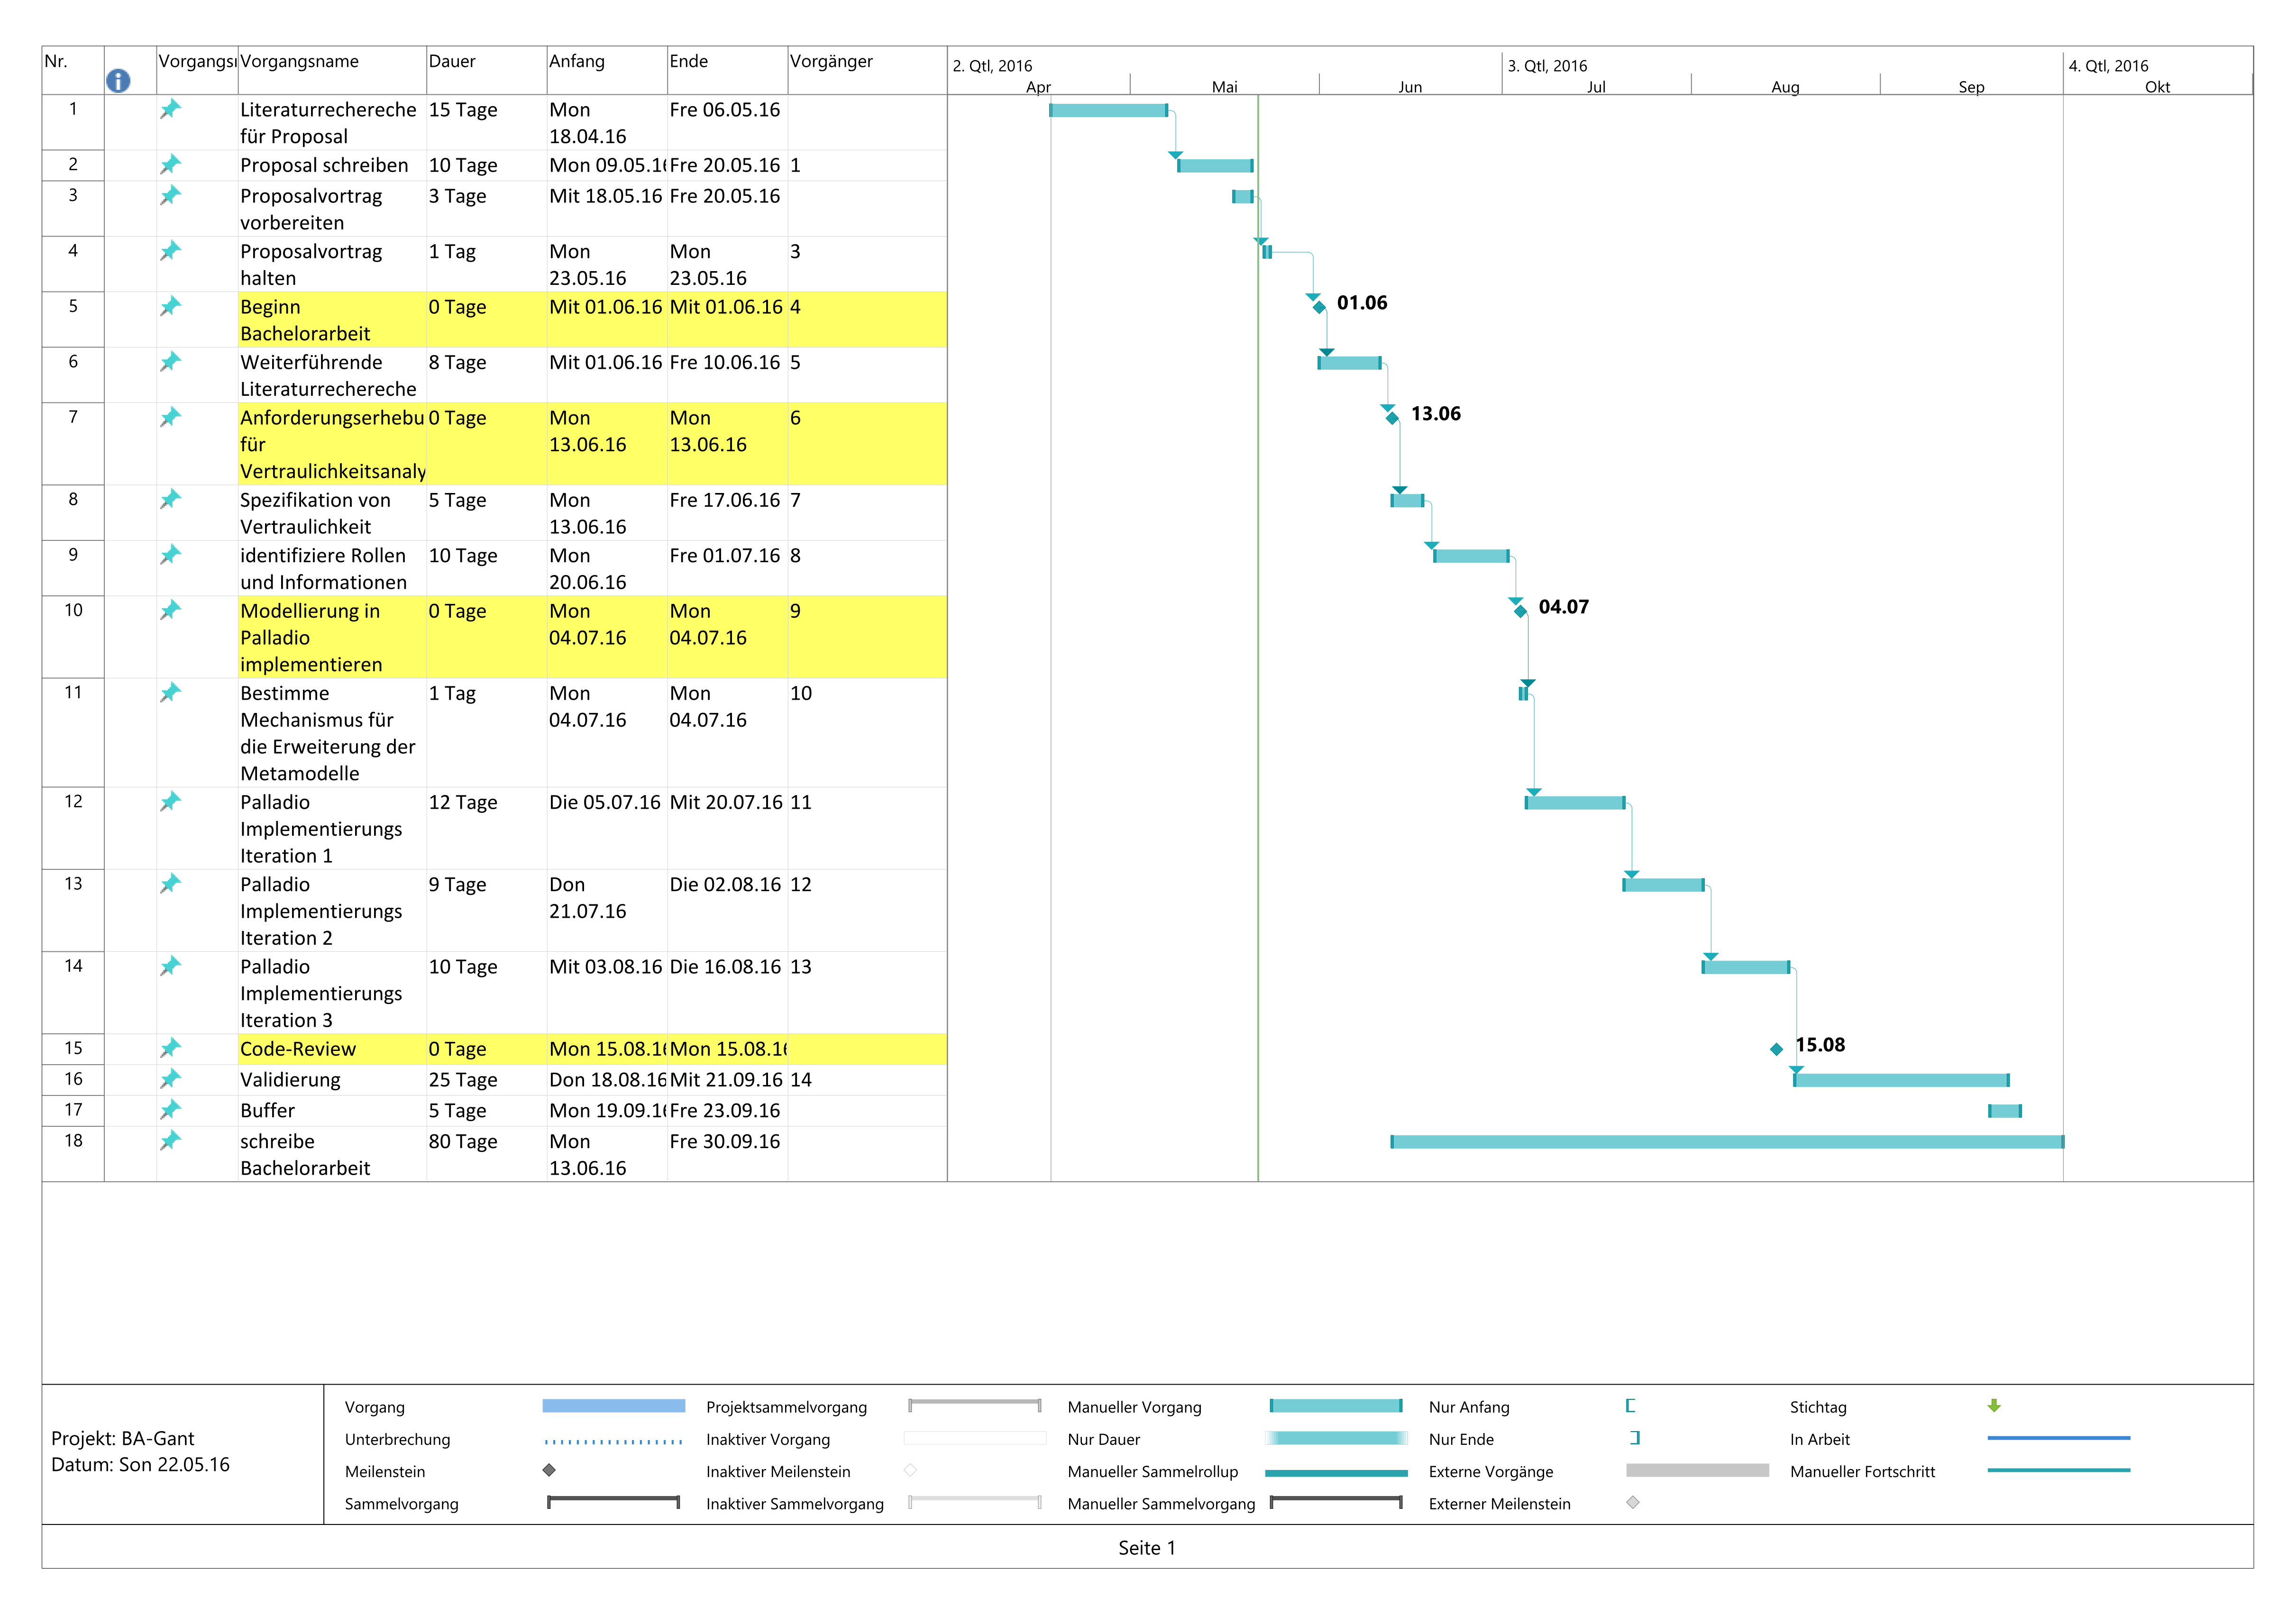
\includegraphics[scale=0.55, angle=90]{images/zeitplan.png}
\label{abb:zeitplan}
\caption{Zeitplan der Bachelorarbeit}
\end{figure}


%% --------------------
%% |   Bibliography   |
%% --------------------

%% Add entry to the table of contents for the bibliography
\printbibliography[heading=bibintoc]


%% ----------------
%% |   Appendix   |
%% ----------------
%\appendix
%%% LaTeX2e class for student theses
%% sections/apendix.tex
%% 
%% Karlsruhe Institute of Technology
%% Institute for Program Structures and Data Organization
%% Chair for Software Design and Quality (SDQ)
%%
%% Dr.-Ing. Erik Burger
%% burger@kit.edu
%%
%% Version 1.1, 2014-11-21


\iflanguage{english}
{\chapter{Appendix}}    % english style
{\chapter{Anhang}}      % german style
\label{chap:appendix}


%% -------------------
%% | Example content |
%% -------------------
\section{First Appendix Section}
\label{sec:appendix:FirstSection}
		
\setcounter{figure}{0}
		
\begin{figure} [ht]
  \centering
  \missingfigure{A figure}
  \caption{A figure}
  \label{fig:anotherfigure}
\end{figure}


\dots
%% ---------------------
%% | / Example content |
%% ---------------------

\end{document}
